\section{Applications}\label{sec:applications}

\subsection{Controller for Virtual Networks}

The most significant DDlog program we have written so far is a
reimplementation of OVN~\cite{ovn} -- a production-grade
virtual network controller used to implement the network substrate
for cloud management systems.

OVN translates a set of network management policies into OpenFlow
rules that have to be installed on the virtual switches in the
network.  The logic is very complicated, comprising tens of input,
output and intermediate relations.

The original program was written in C, and is not fully incremental.
The DDlog implementation has about 6000 lines of code, about the same
size as the original code base, but it is fully incremental.
With the exception of a small number of library functions imported
from C, we were able to implement the entire OVN logic in DDlog.
This would not be feasible with a more traditional dialect of Datalog
that does not support types and expressions, as we relied on these
features extensively in our implementation.

%The original
%program builds an in-memory object model of the database; in that
%implementation joins with a primary key become just pointer
%dereferences.  Moreover, some operations are implemented using
%side-effects and are challenging to do in a declarative model; an
%example is allocation of network addresses, where new addresses are
%allocated using a counter, to prevent old addresses from being reused
%for as long as possible.  The original program generates open-flow
%rules encoded as strings, so this implementation makes extensive use
%of the string interpolation facilities of DDlog.

Preliminary evaluation indicates that the incremental performance is
several orders of magnitude better than the original program for large
networks.  Figure~\ref{fig:ovn_perf} compares the cost of applying a small incremental
change to network reconfiguration for varying network sizes for
C and DDlog versions of the program.

\begin{figure}
    \center
    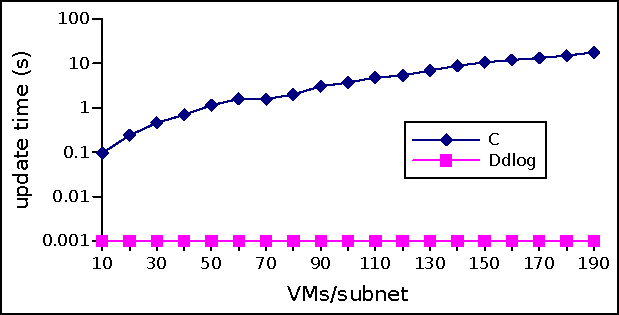
\includegraphics[width=0.4\columnwidth]{update_plot.pdf}
    \caption{The cost of incremental network updates.\label{fig:ovn_perf}}
\end{figure}

%TODO: how well does it work.

\subsection{Program analysis}

We have evaluated DDlog on a large Datalog program written for the
Souffle Datalog compiler.  The Datalog program performs many
compiler analyses simultaneously, computing their fixed-point.  We
have written a Python program that converts a large subset of the
Souffle Datalog syntax into DDlog (we have manually handled the
missing features).  The input program consists of 580 lines, and the
input dataset consists of 3.5 million tuples.

The non-incremental Souffle Datalog engine used by Doop evaluates the
program on this dataset in 23 seconds, whereas DDlog takes 45 seconds.
After the initial evaluation, DDlog propagates small updates, adding or
removing several input records, in under 10ms.  

A hand-optimized version of the program, provided by Doop developers,
reduces the evaluation time to 1 second by using the join order
optimization.  DDlog does not currently allow the developer to
control join evaluation order, which prevents us from reproducing the
same optimization.

%TODO: how well does it work?

%\subsection{Firewall management}
%
%We have reimplemented a proprietary network management application in
%DDlog.  The application manages a firewall in a network of switches
%and virtual machines (VMs).  The firewall is driven by a centralized
%policy.  The centralized policy is implemented in a distributed
%fashion by the VMs and network switches, each of which performs
%filtering using local rules.  When the centralized policy changes, the
%local rules have to be updated in all network devices.  The core
%of this program is a graph reachability problem, which is written in a
%few lines of DDlog.  The DDlog program outperformed a hand-optimized
%Java implementation consisting of several thousand lines of code
%by a factor of 3 to 8.
